\chapter{Theoretical Foundations\label{cha:chapter3}}
This thesis employs multiple different types of deep learning and compression methods, such as \acp{cnn}, self-attention modules, arithmetic coders and the hyperprior architecture. The following sections briefly explain the foundations of these topics in order to aid the understanding of the models proposed in this thesis.
\section{Convolutional Neural Networks}
\begin{figure}[t]
\centering
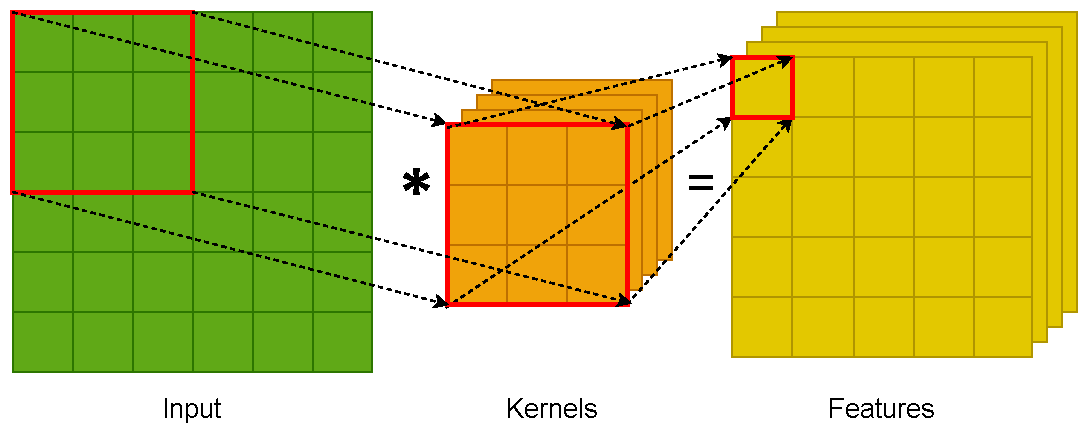
\includegraphics[scale=0.8]{CNN.pdf}
\caption[Example of Convolutional Layer]{Example of a \ac{twod} convolutional layer computing a feature pixel.}
\label{fig:cnn}
\end{figure}

\Acp{cnn} are a type of \ac{ann}, distinguished from other \acp{ann} by the fact that they use convolutional layers as part of their architecture \citep{oshea_introduction_2015}. They were originally designed for image classification, which remains one of the main applications for \acp{cnn} \citep{gu_recent_2018}. However, \acp{cnn} are also used in other fields of machine learning such as \ac{nlp}. The most common type of \ac{cnn} in the field of computer vision uses \ac{twod} convolutional layers in combination with downsampling or pooling layers and activation functions to learn features of an input image. 

A \ac{twod} convolutional layer takes a \ac{twod} image-like input and produces a given number of features each represented as a \ac{twod} matrix \citep{gu_recent_2018}. These features are computed for a given pixel by convolving the neighbourhood of this pixel with a kernel, which is shown in \autoref{fig:cnn}. These kernels are comprised of the weights of the convolutional layer and are therefore learned using gradient descent. A pooling layer is then used to reduce the spatial dimensionality of the input. Such a combination of a convolutional and a pooling layer can be repeated multiple times since the output of both the convolutional layer and most pooling layers are again image-like and can be used as input to additional such layers. Between sets of convolutional and pooling layers nonlinear activation functions are applied in order for the network to be able to learn nonlinear features. The combination of multiple sets of convolutional and pooling layers is central to learning-based image compression and is used in a multitude of the proposed models \citep{balle_end--end_2017,balle_variational_2018,kuester_1d-convolutional_2021,kuester_transferability_2022,guo_learned_2021}.

Compared to other neural network architectures such as \acp{mlp}, \acp{cnn} have low complexity because of the small number of connections between neurons, as each output neuron of a convolutional layer is only connected to a small number of neurons from the input of the convolutional layer, defined by the kernel size \citep{gu_recent_2018}. The low complexity results in \acp{cnn} being resilient to overfitting \citep{oshea_introduction_2015,gu_recent_2018}. However, regardless of the low complexity, \acp{cnn} are still able to learn high-level features of the input because the use of multiple convolutional layers allows for a hierarchical learning of features. This allows the early convolutional layers to learn to detect low-level features such as corners or edges while the later convolutional layers learn higher-level features \citep{gu_recent_2018}

In addition to the \ac{twod} convolutional layer, there are other variations of convolutional layers that are useful, in particular for analysing hyperspectral image data. Firstly, one can define a \ac{oned} convolutional layer, which differs from the \ac{twod} layer in that the kernel moves only in a single dimension. In hyperspectral image analysis, this can be used to learn spectral information, since this information is \ac{oned} \citep{kuester_1d-convolutional_2021,kuester_transferability_2022}. Similarly, \ac{threed} convolutional layers can be defined by using a \ac{threed} cube-shaped kernel. In hyperspectral image processing, this type of layer can be used to learn features of the spatial and spectral domain within a single layer \citep{guo_learned_2021}.

\section{Self-Attention Modules}
The self-attention mechanism is a technique that is widely used in the field of \ac{nlp}. For example, Vaswani et.al. \citep{vaswani_attention_2017} used it as the main part of their proposed transformer architecture which outperformed other machine-learning approaches in various \ac{nlp} tasks at the time, such as language translation. The mechanism aims to compute a latent representation of an input sequence by learning to relate the elements of the input sequence to each other. While a \ac{cnn} can also achieve this, in a \ac{cnn} only elements close to one another are used to compute the latent representation. Using self-attention, the relation of all elements with all other elements can be incorporated, enabling learning of long-distance dependencies \citep{vaswani_attention_2017}.

In recent years, self-attention modules have also been used in computer vision. In image compression for example, self-attention modules can be used in order to enable the neural network to focus on the more complex parts of the input image and subsequently use fewer bits for the compression of the less complex parts of the input, improving the overall compression\citep{cheng_learned_2020, liu_non-local_2019}. 

\section{Arithmetic Coding}
\label{sec:arithmetic}
Arithmetic coding is an algorithm used for entropy coding, that being a technique for encoding and decoding a sequence of symbols in an efficient way \citep{witten_arithmetic_1987}. As an example, a string of characters can be considered. A standard non-optimized method of storing a string is by using the \ac{ascii} encoding which uses a fixed seven bytes per character of the string. Entropy coding algorithms improve on this by allocating fewer bits to more common characters and therefore more bits to less common characters \citep{witten_arithmetic_1987}. In total, this leads to a lower number of required bits for the total message, giving an accurate probability model for the frequencies of the characters. If the provided probability model is perfectly accurate, arithmetic coding yields an encoding close to an optimal encoding, that being an encoding that uses a number of bits equal to the entropy of the encoded input \citep{witten_arithmetic_1987}. This is the fewest number of bits possible for lossless encoding of an arbitrary message, which was proven with Shannon's source coding theorem \citep{shannon_mathematical_1948,mackay_information_2003}.

\begin{figure}
\centering
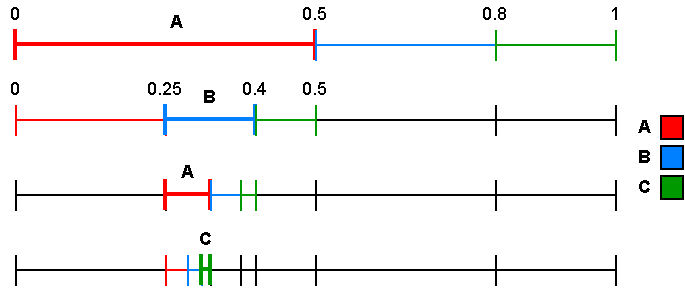
\includegraphics[scale=1]{ArithmeticCoding.pdf}
\caption{Arithmetic Coding Process of the Character Sequence "ABAC".}
\label{fig:arithmetic}
\end{figure}

Arithmetic coding, using the theoretical version of the algorithm, works by encoding the entire input message into one arbitrary-precision rational number $q$ with $0 \leq q < 1$ \citep{said_introduction_2023}. In practice, the algorithm is slightly modified to account for the lack of infinite precision in computers, as will be detailed later in this section. The encoding is performed using an iterative process. To understand this process, consider for example an alphabet consisting of three symbols, 'A', 'B' and 'C' with 'A' having the probability $0.5$, 'B' having the probability $0.3$ and therefore 'C' having the probability $0.2$. Encoding a message is performed symbol by symbol. To encode the first symbol, the interval $[0,1)$ (meaning numbers $a$ with $0 \leq a < 1$) is split into three parts according to these probabilities. If the first symbol is 'A', the final encoding number $q$ will be in the interval $[0,0.5)$. Likewise, if the first symbol is 'B' or 'C', $q$ will be in the intervals $[0.5,0.8)$ or $[0.8,1)$ respectively. The second symbol is then encoded by splitting the interval determined from the first symbol again, using the same probabilities. A sequence of two 'A' symbols would therefore result in $q$ being in the interval $[0,0.25)$. This procedure is iterated until each symbol of the input message is encoded, resulting in a single number $q$ representing the entire input. This process can be seen in \autoref{fig:arithmetic} using the aforementioned probabilities for the word "ABAC". This number encodes the original message nearly optimally given a perfect probability distribution, with a difference of less than a bit to the entropy of the message. The reason for this discrepancy is that $q$ is always represented using an integer amount of bits. If the input image has a non-integer entropy, the required amount of bits to store $q$ is the entropy rounded up to the nearest integer. However, the complete algorithm of arithmetic encoding requires an additional source of information that needs to be transmitted to the decoder. In order to decode the message, the decoder needs to know the probability model as well as a way to distinguish when the message ends. The first is constant with respect to message length. The second can be transferred using only logarithmic overhead with respect to message length. This is often done by adding an additional token that signifies the end of the message \citep{said_introduction_2023}.

As mentioned before, the algorithm is adapted slightly in practice in order to use fixed precision numbers instead of arbitrary precision numbers. Rounding operations as a result of using fixed point numbers are the same for the encoder and decoder and therefore do not inhibit the algorithm in principle. However, as a result of rounding, intervals can become small enough that they are not representable with fixed point numbers of the used precision. In this case, the intervals are changed in a determinable way so that they are again representable. This process is called renormalization and multiple algorithms to perform this procedure exist.
Arithmetic coding also allows for the possibility of changing the probability distribution during the encoding process based on previously encoded symbols. This is possible because the decoder decodes the symbols in the same order as the encoder encodes them and can therefore perform the same change to the probability distribution as the encoder, as long as the method for changing the probability model was decided beforehand \citep{said_introduction_2023}. An example of such an algorithm is \ac{cabac}, which is an entropy coding method used in the video encoding standards \ac{avc} and \ac{hevc} as well as multiple learning-based \ac{rgb} compression models \citep{balle_end--end_2017,balle_variational_2018,minnen_joint_2018}. \Ac{cabac} is a binary encoding method, therefore requiring the data that is to be encoded to be transformed beforehand. It works by using multiple probability models and, for each element that is to be encoded, selecting one of these models based on previously encoded elements \citep{sze_high_2012}. Since the choice of a probability model for each element is only based on elements that were encoded before it, decoding is still possible by performing the same probability model choices as the encoder. Furthermore, the probability models are updated after each encoding step to adapt them to the data.

In learning-based lossy image compression, arithmetic coding is used as part of the Hyperprior architecture order to encode the latent representation of an input image \citep{balle_end--end_2017,minnen_joint_2018,balle_variational_2018}. The latent representation of the input image and the probability distribution used for the arithmetic coder can be learned using \acp{ann}.

\section{Hyperprior Architecture\label{sec3:hyperprior}}
The hyperprior architecture was first proposed by Ballé et al. \citep{balle_variational_2018} to improve on earlier work by Ballé et al. \citep{balle_end--end_2017}, both in the field of grayscale and \ac{rgb} image compression. In the earlier work, a \ac{cnn} using \ac{twod} convolutional layers, downsampling layers and \ac{gdn} as the activation function was used to transform an input image into a latent representation. This network is called the analysis transform. The latent representation is then compressed using an arithmetic coder. Afterwards, another \ac{cnn} is used to transform the decoded output from the arithmetic coder. This \ac{cnn}, called the synthesis transform, is symmetric to the analysis transform in that it contains the same convolutional layers in inverse order. Additionally, instead of downsampling layers and \ac{gdn} upsampling layers the activation function \ac{igdn} is used. The whole model is then trained using a loss function called rate-distortion loss that optimizes compression rate and reconstruction distortion simultaneously. Since the arithmetic coder performs lossless compression and the compression rate of the \ac{cnn} is fixed, optimizing the compression rate corresponds to optimizing the probability distribution estimate of the arithmetic coder and optimizing the distortion corresponds to optimizing the quality of the reconstruction produced by the \acp{cnn}. A disadvantage of this approach is that the probability distribution used for the arithmetic coder is a fully factorized distribution, which is not optimal if the latent representation computed by the analysis transform contains statistical dependencies \citep{balle_variational_2018}.

\begin{figure}
\centering
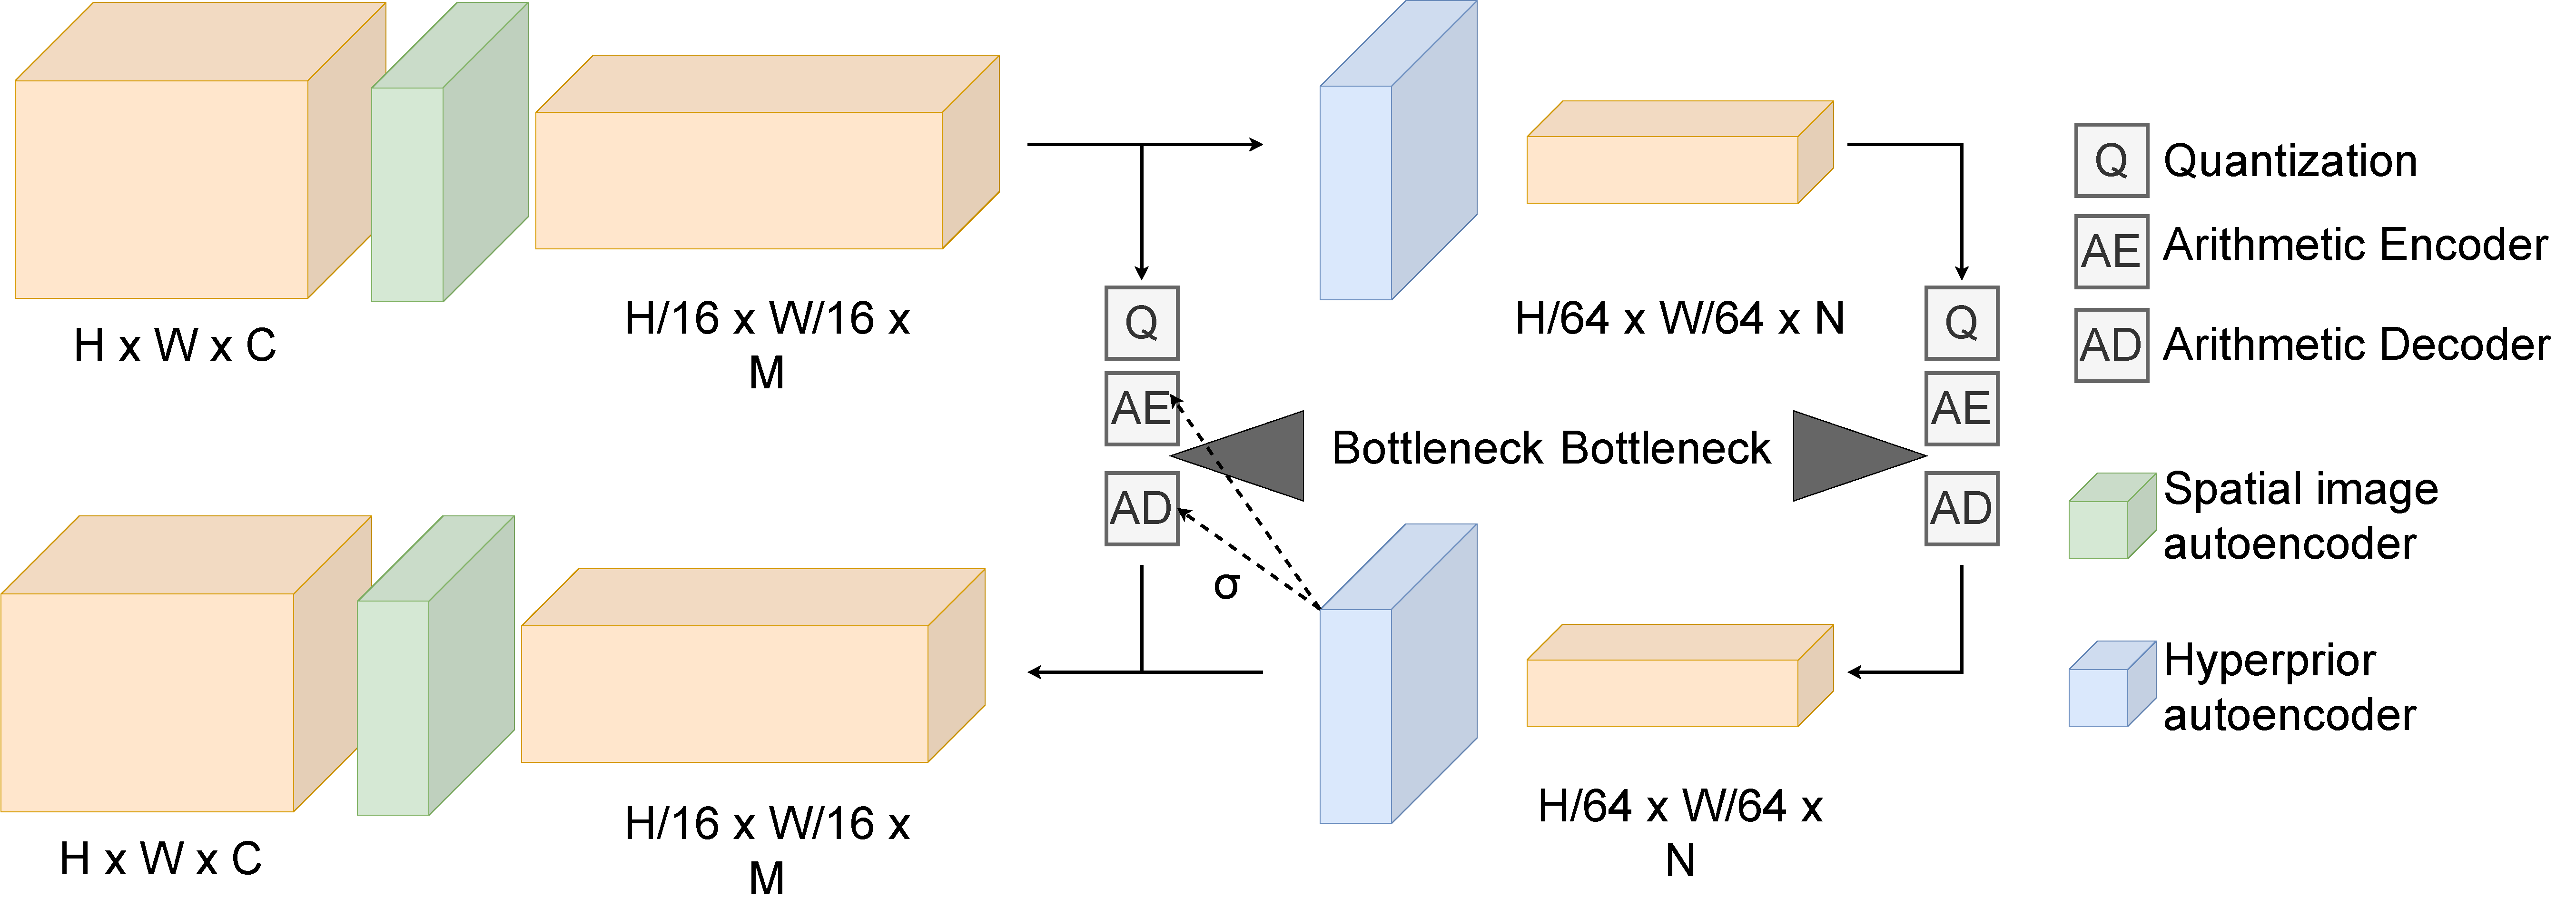
\includegraphics[scale=0.16]{Hyperprior.pdf}
\caption[Scale Hyperprior Architecture]{Architecture of the variational scale hyperprior model proposed in \citep{balle_variational_2018}.}
\label{fig:hyperprior}
\end{figure}

The hyperprior architecture attempts to solve this problem by transmitting information about the probability distribution of the image that is being compressed as side channel information \citep{balle_variational_2018}. This is in contrast to the former model, in which only the probability distribution of the training dataset as a whole is known to both the encoder and decoder. The authors noticed that when modelling the probability distribution with Gaussians, the standard deviations of latent pixels near each other in specific images tend to vary from the overall probability distribution in a similar manner. Note that while the latent vectors are not images, they can be interpreted as images by treating the filters as different channels of an image with multiple channels. In this way it is also possible to refer to pixels of latents, referring then to the values of all filters for a specific point in the spatial dimensions. To address the spatial dependencies of the standard deviations of the latents, an additional \ac{cnn} was added to exploit the spatial dependencies in the latents \citep{balle_variational_2018}. This network is called "hyperprior". The hyperprior network is also split into an analysis and a synthesis transform and is therefore similar to a smaller version of the original \ac{cnn}. A visualisation of this architecture is shown in \autoref{fig:hyperprior}. A difference between the networks is that the hyperprior network uses \ac{lrelu} as the activation function instead of \ac{gdn}. This makes sense because \ac{gdn} is shown to be especially useful for improving visual similarity in an image compression network. This is not useful for the hyperprior network since it does not attempt to learn image reconstruction. Instead, the hyperprior network is used to learn the probability distribution of the latents of the main \ac{cnn}. More specifically, the hyperprior analysis transform produces a bottleneck tensor, which can be compressed with an arithmetic coder using a fully factorized distribution similar to the earlier work by Ballé et al. \citep{balle_end--end_2017}. The hyperprior synthesis transform then predicts the standard deviations for each pixel in the latent of the hyperprior from that bottleneck. This improves the performance of the arithmetic coder significantly because the probability distribution predicted by the hyperprior network is closer to the true distribution than the fully factorised distribution that was used in the model without a hyperprior network. This is especially true if the analysed dataset is heterogeneous, since the fully factorised distribution by definition is the same for each compressed image, while the inclusion of a hyperprior enables the arithmetic coder to use different standard deviations for the distributions of each image that depend on that specific image \citep{balle_variational_2018}. A tradeoff exists in that in contrast to the non-hyperprior approach, the bottleneck of the hyperprior \ac{cnn} has to be transmitted alongside the image data. However, Ballé et al. \citep{balle_variational_2018} showed that the advantage of increasing the performance of the main arithmetic coder outweighs the additional bits of information that have to be transmitted.

\begin{figure}
\centering
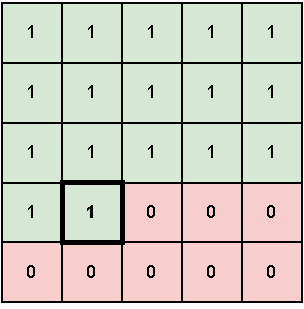
\includegraphics[scale=1]{MaskedConv.pdf}
\caption[Example of Masked Convolutional Layer]{Example of a kernel for a \ac{twod} masked convolutional layer. The pixels to the bottom and right of the current pixel are not used. The current pixel is marked bold.}
\label{fig:maskedconv}
\end{figure}

A further improvement to the hyperprior model was proposed by Minnen et al. \citep{minnen_joint_2018}, seen in \autoref{fig:hyperpriorcm}. They first added a context model to the main arithmetic encoder. This context model adjusts the probability distributions for a specific image during the decoding process based on the already decoded elements. This is a common approach in arithmetic coding \citep{said_introduction_2023}. See also \autoref{sec:arithmetic} for more elaboration on this idea. While the arithmetic coder in the previous models was based on the \ac{cabac} algorithm and therefore also context-sensitive, the context model did not improve the model significantly because images that were to be compressed were fed into the autoencoder sequentially pixel by pixel, which is not optimal \citep{balle_end--end_2017}. Minnen et al. improves the context model by introducing a masked \ac{twod} convolutional layer applied to the quantized latents of the main \ac{cnn}. A masked convolutional layer in this case refers to a convolutional layer in which the kernel only contains pixels up and to the left of the currently transformed pixel. This idea, first proposed in Oord et al. \citep{oord_conditional_2016}, ensures the layer only uses the parts of the input that are at this point known to both the arithmetic encoder and decoder. If a standard convolutional layer were used, the output of the arithmetic coder would not be decodeable, since it would be partly based on pixels that are not yet decoded.  The output of this layer is then combined with the output of the hyperprior synthesis transform using a three-layer \ac{cnn} with 1x1 kernels to produce the parameters used for the arithmetic coder. Since the inputs to the context model can also be seen as coming from the output of the arithmetic decoder because of the losslessness of the arithmetic coder, the context model can be seen as an autoregressive component improving the probability distribution estimates of the arithmetic coder \citep{minnen_joint_2018}. The other improvement proposed in Minnen et al. \citep{minnen_joint_2018} is a change from a Gaussian scale hyperprior to a \ac{gmm}. In contrast to the hyperprior in Ballé et al. \citep{balle_variational_2018} that predicted only the standard deviations of the Gaussians, the proposed model also predicts the means of the Gaussians. This is achieved in the model architecture by making the number of filters in the last layer of the hyperprior synthesis transform and the number of filters in the masked convolutional layer of the context model double the number of filters in the output layer of the main decoder. In this way, for each element in the latent two values in the probability distribution are predicted, the mean and the standard deviation \citep{minnen_joint_2018}.

\begin{figure}
\centering
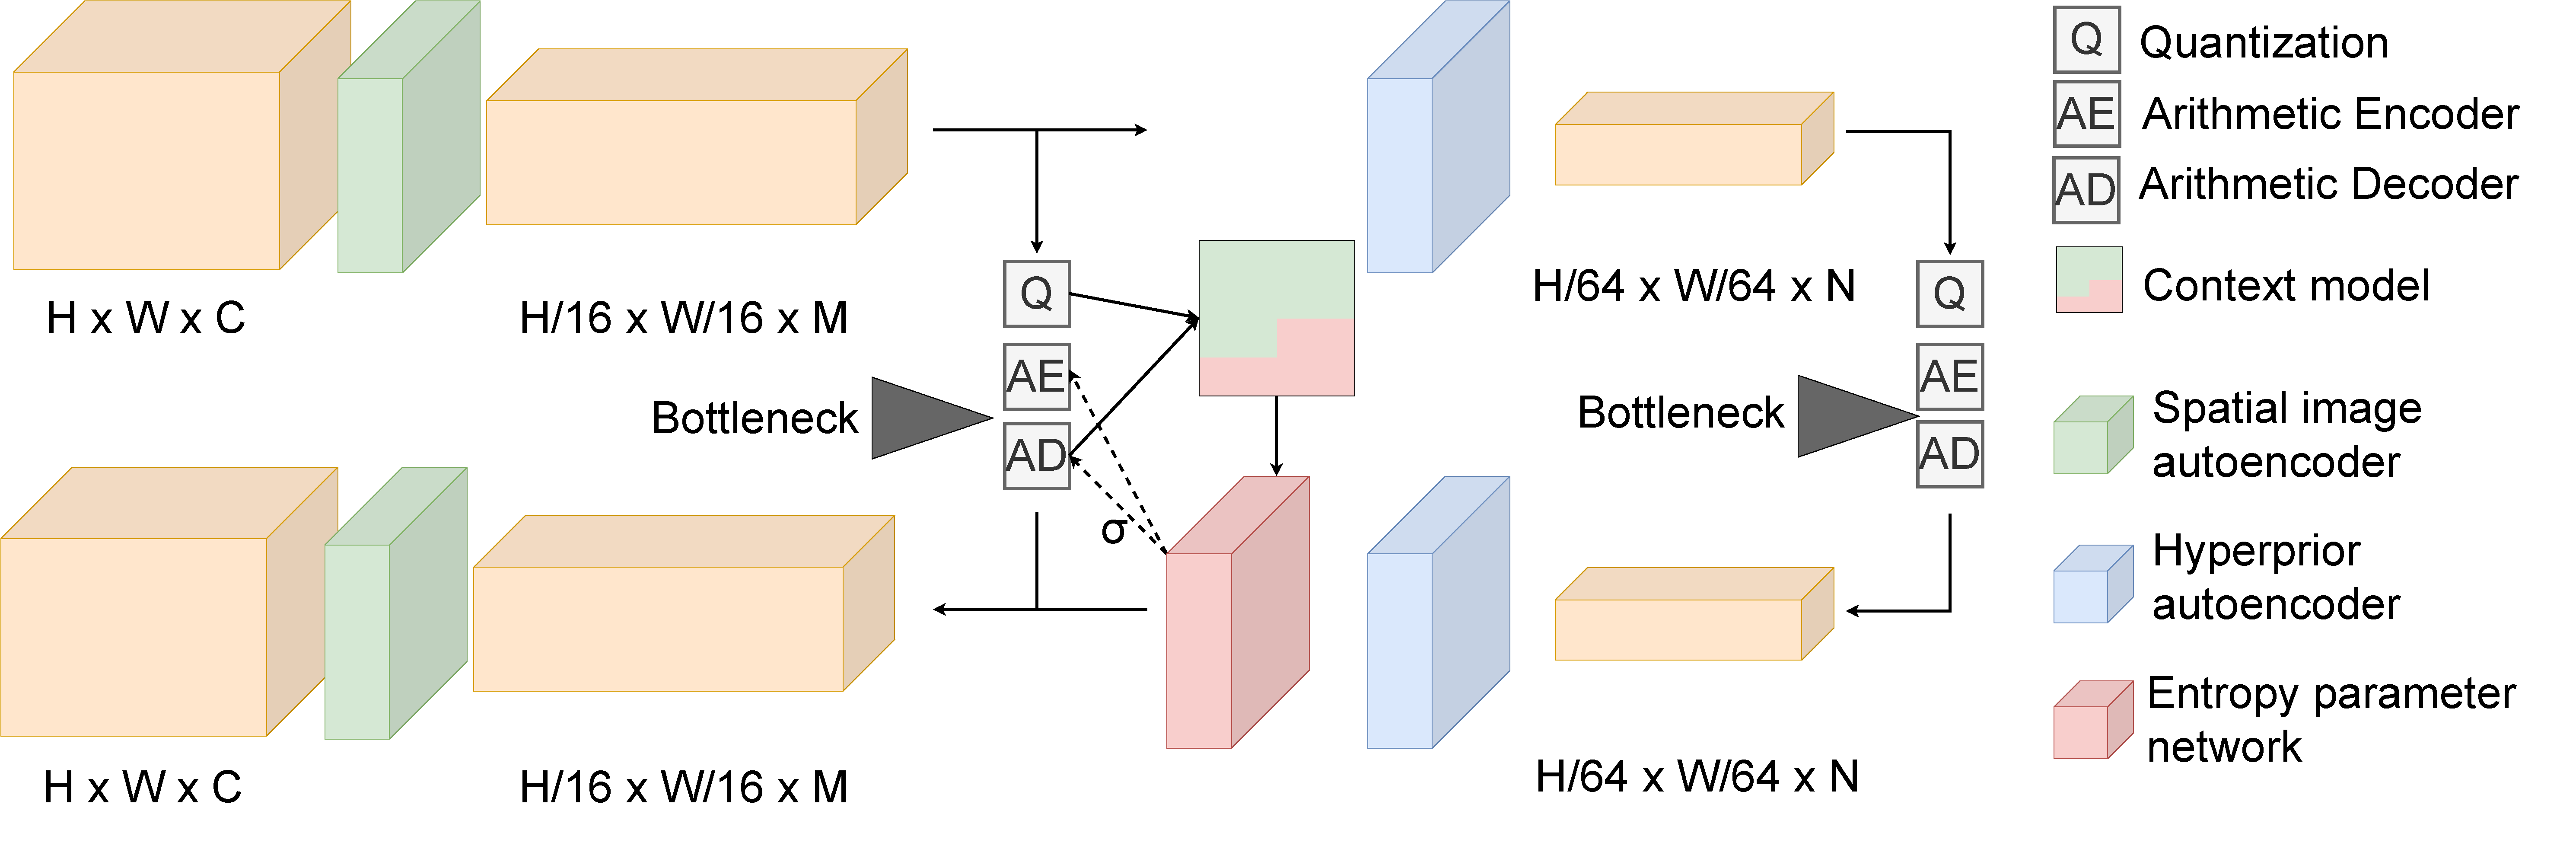
\includegraphics[scale=0.16]{Hyperprior_CM.pdf}
\caption[Joint Hyperprior Architecture]{Hyperprior model using an autoregressive context model proposed in \citep{minnen_joint_2018}.}
\label{fig:hyperpriorcm}
\end{figure}
